\documentclass[12pt, A4]{report}
\usepackage[utf8]{inputenc}
\usepackage{graphicx}
\usepackage{upgreek}
\usepackage{subfig}
\graphicspath{ {images/} }
 
\title{Assignment OOP}
\author{Franklyn Josef Sciberras (0441498(m))}
\date{Friday 12 January}

\begin{document}

\begin{titlepage}
\pagenumbering{gobble}
\maketitle
\end{titlepage}

\pagenumbering{arabic}
\chapter*{LegOOPolis}
	\section*{Analysis of the problem}
	In this section we were assigned to build a program which takes as an input a csv file which contains a number of lego pieces to be stored as stock, and a number of buildings to be built. Then the program needs to attempt to build these buildings using the available stock. In the following sections, one can find the approach undertaken. 

		\subsection*{csv\_reader}
		The first step to take was that of translating the commands found in the csv file into commands readable by our program. In order to do this, the class provided was used and modified to our needs. From such class we would achieve parsed values which are then stored as local variables and then passed to other classes which will be described in the following sub sections.

		\subsection*{Quarry}
		The first three values to be stored are those of the amount of bricks, windows and doors available in stock. However in order for this stock to be stored, we needed something to store them. Just like in real life, a quarry was built. The job of this class was to create three linked lists in which we could store the pieces (will be explained in the next section). Then Lego\_Factory (will be explained in another sub-section)would be called in order to provide us with the necessary amount of pieces and then store them. Also this class has the functionality of providing other classes, with the amount of each lego piece remaining, and removing the necessary amount of lego pieces from it. A singleton design pattern was used since it was deemed fit that only one quarry can be available, such that the builders wouldn't have to worry about from which quarry they would need to get their lego pieces.

		\subsection*{Linked\_list and node}
		These two classes apply a generic approach, where we could define one type which will be stored in them at initialisation, and then we would be able to store that type of object in them, without having to use method overriding. In order to do so, generic programming was used along with the creation of nodes. We would be storing the object in the node and the linked list would have a pointer to the beginning of it and another one to the last node created. Each node would contain a reference to the object that will be stored and a pointer to the next node. Finally the Linked\_list class would contain various methods which would enable us to create new entries, delete other ones as well as show the amount of objects a specific linked list of a specific type, is storing.

		\subsection*{Lego\_piece and its Sub Classes}
		This class is a generic class which represents the tree type of pieces which will be available to our software, them being; Brick, Door, Window (all three of them were created as sub classes, which extend from Lego\_piece as a parent class). However we can never have an instance of a generic lego piece since this doesn't mean anything in the scope of our software. For such reasons this class was made an abstract. Even more trough such an approach we would able to take a polymorphic approach when dealing with lego pieces.

		\subsection*{Lego\_Factory}
		Seeing that a numerous amount of different lego pieces would be needed throughout the software, Lego\_Factory class, which implements the factory design pattern, was created. This class serves as an intermediary class, which is supplied with the type of piece that is needed, and returns an instance of that specific piece.

		\subsection*{Building and its Sub Classes}
		This class is a generic class, which represents all the different kind of buildings that can be built in our software, with them being; 1 storey building, 2 storey building, church, hospital and university (where all 5 of them were created as sub classes which extend from Building as a parent class). However we can never have an instance fo a generic building, since it doesn't make sense for a builder to build a building of a generic type. For such reason, building class was made as an abstract. Opting for such an approach, we would be able to use polymorphic transformations when dealing with buildings. 

		\subsection*{Building\_Factory}
		Seeing that a numerous amount of different buildings would be needed throughout the software, Building\_Factory class which implements the factory design pattern, was created. This class serves as an intermediary class, which is supplied with the type of building that needs to be built and returns an instance of that specific building.

		\subsection*{Builder and its Sub Classes}
		This class is a generic class, which represents all the different kind of builders that can build our buildings, with each building having a specific kind of builder that can build it. However these builders cannot build the buildings themselves. They need to have contractors which enable the actual building of the buildings. In all we have three contractors, with them being: 
		\begin{enumerate}
			\item Bob
		 	\item Peter
		 	\item Jane
		\end{enumerate}
		\par
		These three contractors however are only to build specific buildings. For example, contractor Bob is only able to build 1 and 2 storey buildings, whereas Peter is only able to build churches, whereas Jane is able to build universities and hospitals.
		\par
		This type of design required a multiple inheritance approach, however due to its shape, requirements and nature, the diamond problem arised. In order to be able to deal with this problem, our specific builders inherited in a virtual manner from the Builder class, whereas the contractors inherited normally from them. In doing this we only got a single instance of class Builder in the contractor classes, whereas if the inheritance was a normal one, we would have had two instances of the class Builder in our contractor classes. 
		\par
		Even more in our contractor class, we included a dummy method for build(), which overrides the inherited once, just to conform with compiler specifications. However since such method was never needed, (since in contractor class we would call the appropriate method from the appropriate parent class, according to the type of building being built). In order to make such a method inaccesible, since it was not of use, we set it to private.
		
		\subsection*{City}
		This class was used to store the succesfully built buildings and generate a report about the requested amount of buildings as well as the ones we managed to build. Also in order to be able to store such buildings, an instance of a linked list was initialised in the form of Buildings. This enabled us to store all the different kind of buildings in one data structure using polymorphism.

		\subsection*{LegOOPolis}
		Finally the main class was built. In this class we stored the parsed commands from the csv input file locally, by initialising the csv\_reader class and passing the location of the input file to it as a parameter from command line arguments. Then the main class would ask for a reference to the singleton instance of Quarry and give it its stock count. Then the building contractors Bob, Peter and Jane would be initialised and asked to build the necessar buildings. In doing so they would check if enough material is present in the quarry and if yes build the building. Such building would then be stored in the city instance which we create. After all the buildings are attempted a report of the outcome is generated, and cleanup of memory commences, in order to respect memory management protocols.

	\section*{Testing Cases And Results}
	After examining the approach undertaken in the previous two sections, we had to test the produced code under various test cases. In this section we will be describing the different test cases used and analising the produced outcome. 

		\subsection*{Correct Input Testing}
		The first test carried out was correct input testing. In this section we wanted to make sure that when our software recieves a file with valid input, it performs as expected. Here two factors were taking into consideration:
			\begin{enumerate}
				\item All the buildings requested were attempted
				\item Builders did not build any buildings if there wasn't sufficient material
			\end{enumerate}

			\begin{figure}[h]
				\centering	
				\subfloat[Input]{{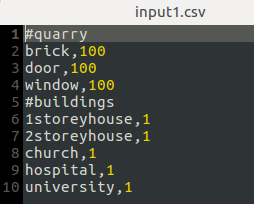
\includegraphics[width=3cm]{input1}}}
				\qquad
				\subfloat[Output]{{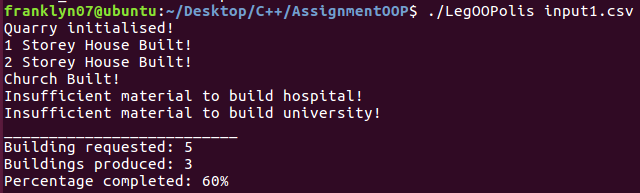
\includegraphics[width=9cm]{input1Test}}}
			\end{figure}

		\subsection*{Invalid Input Testing}
		The second test was about testing how the software would perform when given a file as an input with an out of the norm format. In this section we wanted to make sure that the file was parsed correctly and only valid commands were attempted and stored. From the following screenshot you can see that only the university building was a valid command, however there was no valid command whith regards to stock intake, thus the university could not be built. The rest of the commands were invalid, thus no more attempts to build buildings were made.

			\begin{figure}[h]
				\centering	
				\subfloat[Input]{{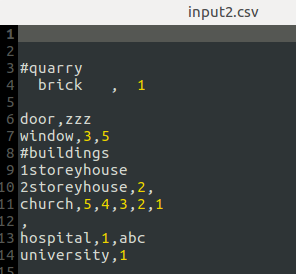
\includegraphics[width=3cm]{input2}}}
				\qquad
				\subfloat[Output]{{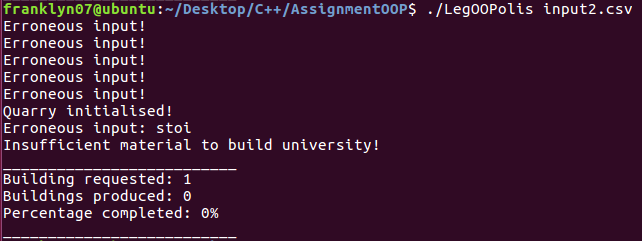
\includegraphics[width=9cm]{input2Test}}}
			\end{figure}

		\subsection*{Attempting To Build New Types of Buildings}
		The third test was about testing whether the software would proceed gracefully if the input file requested a type of building which was not described in the specifications. From the following figures, one can notice that such buildings were not taken into account and the software proceeded as if such commands were not present.

			\begin{figure}[h]
				\centering	
				\subfloat[Input]{{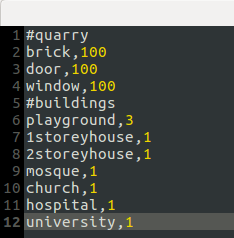
\includegraphics[width=3cm]{input3}}}
				\qquad
				\subfloat[Output]{{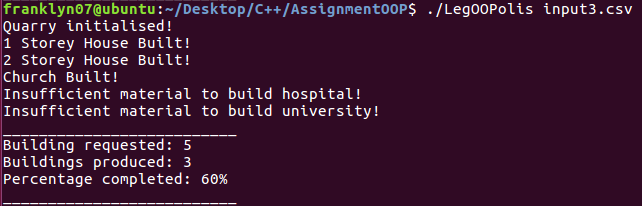
\includegraphics[width=9cm]{input3Test}}}
			\end{figure}

		\subsection*{Attempting To Add New Types Of Lego Pieces To The Quarry}
		The final test was about about trying to add new lego pieces to the quarry. Since such lego pieces would be undefined, we wanted to see how the software would react and whether it would break or not. The figures below show that such inputs were ignored and the software proceeded gracefully in performing its expected job.

			\begin{figure}[h]
				\centering	
				\subfloat[Input]{{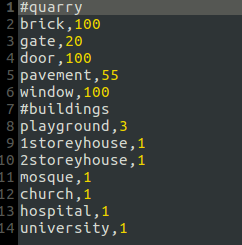
\includegraphics[width=3cm]{input4}}}
				\qquad
				\subfloat[Output]{{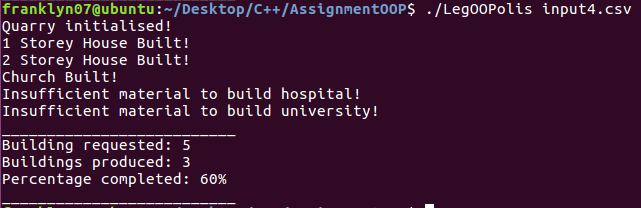
\includegraphics[width=9cm]{input4Test}}}
			\end{figure}

	\section*{Critical Evaluation And Limitations}
	After testing out the produced software, there were a couple of areas in which one could improve, that were noticed.
	In this section we will be discussing these limitations.

	\par
	The first kind of shortcut that was taken in the approach of building such an implementation, was that of storing each type of lego piece in a seperate linked list. In doing so, we facilitated a lot of computational work as well as needed algorithms, when it comes to checking whether there is sufficient material needed or not and when it comes to deducing material from the quarry. 

	\par
	Even though this is computationally more efficient, since you don't have to traverse the whole single linked list to achieved the previous mentioned situations, it does not mimick real life situations. Where most of the time a box of lego pieces, contains the different types of lego pieces all jumbled up together. However in such a case computational efficiency wsas preferred over real life mimicking.

	\par
	Another situation was that of when a builder attempted to build a building. In order to achieve the building, the software first initialised the desired building (and in doing so, it was assuming that the building was already built), and then checking if there are enough pieces in the quarry to build it, and if there were; the building was added to the city and the required materials reduced from the quarry. If there weren't sufficient resources, then the building was deleted whilst the pieces were not remove at all from the quarry. 

	\par
	This also doesn't mimick real life events, since a building cannot be built if there aren't sufficient materials to build it. However such an approach facilitated the way we reasoned about the building of buildings, and even more fulfilled a side condition that pertained to the assignment, which required of us to think of a way how to address the issue of returning pieces to the quarry, which were going to be used, however due to limiations of other pieces, the building could not be built, thus they were not needed any more.

	\par
	Finally, it was noted that some methods where not needed outside of the scope of the specific class and thus they should have been made private in order to restrict access as well as to enhance encapsulation. However this was noticed at a very late stage of the software production, and due to time constraints they were left as they where.


	\section*{Final Discussion}
	In this section I will be discussing the reasons behind the specific design choices I made. Even more, some points with regards to the use of abstraction, encapsulation, polymorphism and inheritance as tools to make the design more concise and more OOP oriented, will be made.

		\subsection*{Design Choices}
		If one examines the UML diagram produced, as well as the Analysis Of The Problem section and how the problem was tackled, one could notice the two design patterns included. These were the Singleton design pattern and the factory design pattern.

			\subsubsection*{Singleton Design Pattern}
			From our problem specifications, I could notice that there would only be one quarry at a time, which would contain all of our resources, and all of our builders would be taking materials as need be from it. Since only quarry could exist per instance of the problem, Singleton design pattern was deemed fit to build such class. In doing so, it was ensured that only one quarry instance would be occurring at a time, and thus there wouldn't be any issue when it comes to storing and retrieving stock. However keeping in mind future development of the software, it was decided that the builders would recieve a pointer to a quarry in order to get their resources, rather than a hardcoded reference to the instance. In doing so, if in future development, one would need to instill more than one type of quarry, this could be done, without having to manipulate most of the code.

			\subsubsection*{Factory Design Pattern}
			Another pattern that was observed in the analysis and design of an approach to the problem, was that we would be having multiple instances of lego pieces and buildings. In order to facilitate such creation of instances of the different lego pieces and buildings, the Factory design pattern was implemented both for the Building class as well as the Lego\_piece class. In doing so, we would only have to specify to the factory what specific building or piece we would be needing and in turn it would return to us an instance of that building or piece.
			
			\subsubsection*{Extra Functionality}
			As instructed in the assignment description, if the quarry didn't have the required amount of pieces to build a building, the lego pieces already taken out of the quarry need not be returned to the quarry (for simplicity's sake). However in the previous section, we talked about how such issue was tackled and actually pieces which were not used since a building was not built, were still kept in the quarry.

		\subsection*{OOP Principles}
		Besides the previously mentioned design choices, the four basic OOP principles (that are; Encapsulation, Abstraction, Polymorphism and Inheritance) were used throughout, in the design of such software. However in this section we will emphasize more on two aspects of OOP which are a trait of the C++ language.

			\subsubsection*{Multiple Inheritance}
			If one observes the UML diagram, in the builder section, one could notice that the contractor classes, mainly Bob and Jane inherited from more than one class. This type of behaviour is synonym with the C++ language and is called multiple inheritance. Such a behaviour allows a class to inherit variables and methods from multiple classes, and thus it would avoid the need of having to write duplicate code, or excessive method overriding (as its the case whith java when using interfaces to mimick multiple inheritance), in order to include all the required methods. It also enhances polymorphism, where methods can be declared on the generic type of class and then the specific return/parameter needed would be decided at run time (as long as its an instance of an inheriting class). However two problems arise with this type of inheritance; if the class inheriting, inherits two methods with the same name, how would it know which one to keep and which one to discard. Even more if the classes it is inheriting from, are inheriting from the same parent class, the sub class where multiple inheritance is occurring, would recieve multiple instances of the super class. In order to solve these problems, the following approach was taken:

				\begin{enumerate}
					\item  Since we needed both inherited methods to be available in the contractor class, even though they had the same name, we created an overriding dummy method, which was set to private to be inaccessible, as an overrider. Then whenever we needed a specific inherited method, we would call it through the class it was situated in (ex. jane.university\_builder.build()).
					\item In order to have only one instance of the super class, in the child class, the classes immediately inheriting from the super class, inherited virtually. In doing so, only an instance woulde be present of the super class in the child class (Diamond problem).
				\end{enumerate}
			
			\subsubsection*{Memory Management}
			Another charactersitic of the C++ language, is that whenever an instance of an object is going to be deleted, the destructor needs to be called. By default the destructor method is empty, however in order to be able to give back resources to the machine, we have to manually delete any objects created which have become useless to the general scope of the process, in the destructor method. This is done since in C++ there is no automatic garbage collector and thus memory has to be retrieved manually, in order not to clog the system. In doing so memory leaks will be prevented, making the program consume only the necessary amount of resources needed. Note that whenever an inheriting class' instance will be deleted, it will always call its super class destructor.

\chapter*{KasparOOP Chess}

	\section*{Analysis of the problem}
	In this section we were assigned to build a chess game which as an input takes a csv file that contains an arbitrary set of chess moves in the following format: $<PLAYER>,<COMMAND\_TYPE>,<SOURCE>,<DESTINATION>$, where player can either be black or white, command type can either be 'move' or 'eat' and the co-ordinates are given in the format 'c1'. In the following sections, one can find the approach undertaken.

		\subsection*{InputReader}
		\par
		The first step to take was that of translating the commands found in the csv file into commands that our program could read. In order to do that, InputReader was created. This class would be given an input file as a parameter and tokenize it using the delimeters $'<', '>' and ','$. Then the values achieved after removing such delimeters would need to be stored, with each line being a seperate command, and each command being stored in an array list. However since no primitive data structure exists which could hold a collection of strings and integers, class Command was created to cater for this(it will be explained in the next sub section).\\

		\par
		However the values achieved still wouldn't be in our desired form. For such reasons a Utility class was created in order to translate the obtained commands into the desired ones (class will be explained in greater detail further on). Since it is easier to work with integers rather than characters, the source and destination command would be parsed into two seperate integer x and y co-ordinates. Then these would be stored in the Command class along with the player turn (aka. player) and the command type.\\

		\par
		In order to cater for bad user input, multiple try and catch blocks were introduced, such that bad commands wouldn't be parsed. For example commands with more than 4 fields were ignored, as well as commands with the player turn was something different rather than 'b' or 'w' and moves which included something different than 'move' or 'eat'. Even more, co-ordinates which were out of reach of the boards size, would also be ignored and not parsed.

		\subsection*{Command}
		This class would act as a data type. Attributes obtained from parsed commands where stored in the appropriate primitive data type fields, with them being player, command, source x and y co-ordinates (seperate), destination x and y co-ordinates(seperate).

		\subsection*{Utility}
		As explained in a previous section, this class would serve to perform all the necessary translations. It would facilitate user interface by on screen showing co-ordinates in the form inputted, however internally it would be translating everything to easier to deal with integers. Moreover this class would include a function which would check for any co-ordinates which would be out of bounds and eliminating them. This will be very handy in the Move class.

		\subsection*{Game}
		This class would be the main game engine. Here 2 instances of Player would be created, one being black and one being white, and the Board class instance is also requested. Then the list of parsed commands is passed as a parameter, where the engine would start checking each move's validity. This time validity would not be compromised by bad syntax, but by bad logic. Situations this class checks for are:

			\begin{itemize}
				\item The command being executed is of the correct player during his turn
				\item The piece the player is moving is his
				\item The piece movement is a valid move (eg. Bishop moves only diagonally)
				\item For all the pieces except for the knight, there is no blocking piece when a move will occur
				\item The source co-ordinate is not empty
				\item The destination is empty on move
				\item On eat, the move is a valid move, as well as the destination contains an opponent's piece
				\item Whether king has been eaten, resulting in check mate.
			\end{itemize}

		\subsection*{Player}
		Player class was used in order to represent players playing the chess game. Each player would have his set of pieces, which he then puts on the board. The player pieces would have a colour based upon the players colour, which would be spcified upon construction. Note also that players know when is their turn, and to be linear with chess rules, white player always starts the game. This property is stored in a boolean field called myTurn.

		\subsection*{Piece}
		As specified in the previous sub section, each player would have his set of pieces. However there are 6 kind of pieces, which mainly all share the same properties and functions. It can also be concluded that a generic piece does not exist, and must be of a certain type. For these reasons abstract class Piece was created which would represent the general functionality and attributes of pieces, without the ability of being initialised. Note that every piece is able to generate his possible moves, however not every piece has the same possible moves. Thus, the abstract method possibleMoves, was created which would then be overriden in the specific extending classes(aka. bishop, king, queen and so on), where the appropriate function from the class Moves, would be called respectively. Note that the classes extending Piece will not be explained seperately, since they all do the same thing; that is they store their appropriate colour, symbol and value, and call the appropriate move function to generate their possible moves.

		\subsection*{Moves}
		This class takes care of generating the possible move co-ordinates for every single piece, by getting their starting position and implementing respective algorithms to produced all the possible outcomes that conform to the rules and storing them in an arraylist. In order to limit such an outcome to only co-ordinates present on the board, Utility class is used. Since no primitive data type is able to store x and y co-ordinates in a single object, the data type Co\_Ordinate was created.

		\subsection*{Co\_Ordinate}
		Co\_Ordinate handles all the co-ordinates generated by Move, by storing the x integer and respective y integer, in a single component, making it easier to deal with moves.

		\subsection*{Colour}
		As mentioned in the previous sub sections, both players and pieces make use of a colour, which is either black or white. It is very tedious for us writing the game, to be dealing with strings every time, in order for the program to recognize the player and piece colour. For such reason the enumaration class Colour was constructed, in order to facilitate the process.

		\subsection*{Board}
		In order to be able to play the game, there must be some data structure which stores the pieces in their current location. To achieve this, Board was constructed. Since a chess board is made up of 64 boxes which actually themselves hold the piece, class Box was constructed (will be discussed in next sub section) and a 2d array which holds these Box structures was implemented. However we wanted to make sure that only one board was present per game (since it wouldn't make sense otherwise). Thus the singleton building pattern was adapted. In order for the user to be able to visually see the current Board status, the paintBoard functionally was also introduced. 

		\subsection*{Box} 
		The data type Box was constructed in order for it to hold the piece itself. Since in all there will be 64 boxes, from which some will be empty, and others will be containing pieces, we wouldn't want them to be mixed up, since this would change the game status. Thus the co-ordinate that they are assigned at first, when they are stored in the 2d array, is binded to them permanently using final variables to store their respective co-ordinate.
		
		\subsection*{Observer Classes}
		Since every game needs to be won, and user interaction was not in realtime, we had to come up with a point system, which would deduce the winner of the game, after execution. In order to keep track of the points being won by each player as well as other statistics, the observer design pattern was implemented. Two interface classes were used to define the functions which would be adapted by the Subject and Observer respectively. Then GameWatcher was constructed which would implement the subject interface, where it would be watching the game and notifying all the observers watching the game of any updates. Evenmore PlayerObserver was constructed in order to define the functionality of the observer, such that player statistics would be stored (implements Observer). 2 instances of this class would be registerd in the Game; one for the black player and one for white.

		\subsection*{PlayerReport}
		Since match statistics per player have been collected, these need to be displayed for the user to see them as well as for the game engine to decide a winner. Thus PlayerReport is created and used in the game engine, such that when the whole command file is executed, each players statistics as well as those of the game are displayed on screen, using a method in the game engine, called gameReporter.

		\subsection*{KasparOOP}
		KasparOOP is the main class, which ties everything together. It instantiates the game and starts it, with the cammand file to be executed, firstly being passed to  InputReader through command line arguments (for parsing), and then to the game instance. KasparOOP also handles any errors related to the file opening and closing.
	 
	\section*{Testing Cases And Results}
	After examining the approach undertaken in the previous two sections, we had to test the produced code under various test cases. In this section we will be describing the different test cases used and analising the produced outcome. 

		\subsection*{Turn Based Testing}
		The first test carried out was turn based testing. In this section two factors were put under test, mainly:
			\begin{enumerate}
				\item Testing that the game is turn based - player cannot move 2 times
				\item Testing that the player cannot move another players piece during his turn
			\end{enumerate}

			\begin{figure}[h]
				\centering	
				\subfloat[Input]{{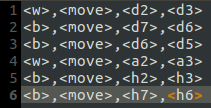
\includegraphics[width=3cm]{turnBasedTestCommands}}}
				\qquad
				\subfloat[Output]{{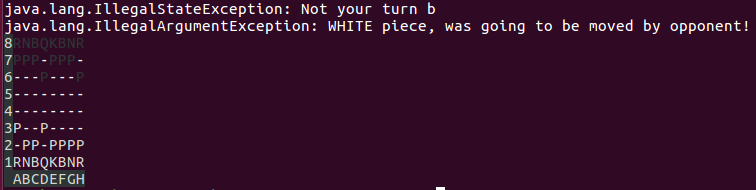
\includegraphics[width=9cm]{tbs}}}
			\end{figure}

		\subsection*{Move Functionality Testing}
		The second test was about the move functionality. In this section the following two factors were put under test:
			\begin{enumerate}
				\item Moving all pieces using valid and invalid moves (eg. Rook moving diagonally)
				\item Trying to move a piece whilst its blocked
			\end{enumerate}

			\begin{figure}[h]
				\centering	
				\subfloat[Input]{{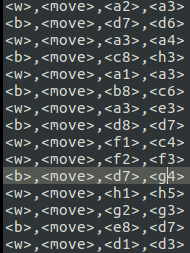
\includegraphics[width=3cm]{moveFunctionalityTestCommands}}}
				\qquad
				\subfloat[Output]{{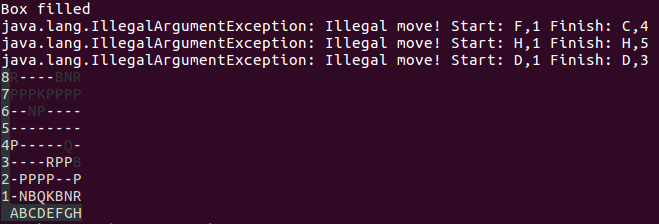
\includegraphics[width=9cm]{mfts}}}
			\end{figure}

		\subsection*{Eat Functionality Testing}
		The third test was about the eat functionality and the following factors were put under test:
			\begin{enumerate}
				\item Try to eat from an empty box
				\item Try to eat a piece from your set
				\item Try to eat using a valid move (for each piece)
			\end{enumerate}

			\begin{figure}[h]
				\centering	
				\subfloat[Input]{{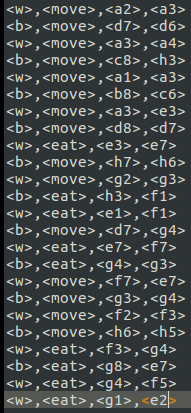
\includegraphics[width=3cm]{eatFunctionalityTestCommands}}}
				\qquad
				\subfloat[Output]{{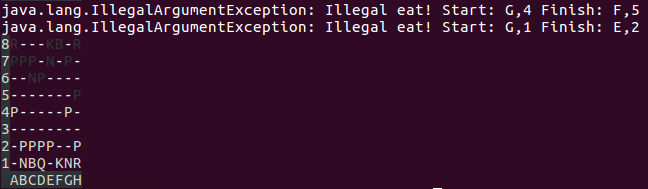
\includegraphics[width=9cm]{efts}}}
			\end{figure}

		\subsection*{Bad Command In Input File Testing}
		The final test was about bad inputs in the input file. The following eventualities were tested for:
			\begin{enumerate}
				\item Have extra commands (eg. 5 commands rather than 4)
				\item Input an illegal colour
				\item Input an illegal move
				\item Try to reach an unreachable box
			\end{enumerate}

			\begin{figure}[h]
				\centering	
				\subfloat[Input]{{\includegraphics[width=3cm]{badCommandsTestCommands}}}
				\qquad
				\subfloat[Output]{{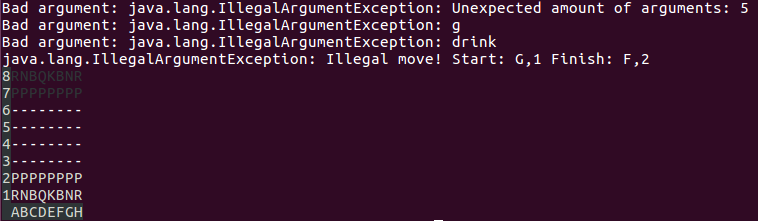
\includegraphics[width=9cm]{bcts}}}
			\end{figure}

	\section*{Critical Evaluation And Limitations}
	After testing out the produced software, there were a couple of areas in which one could improve, that were noticed.
	In this section we will be discussing these limitations.

	\par
	Firstly, it was noted that the pawn could not move two boxes from the starting piece. This violates the chess rule, that when a pawn is found on the starting box, it can move one box or two boxes forward.

	\par
	Secondly, the parser was limited when it comes to source and destination commands which didn't comply with the supposed form. If the source or destination contained a third character (or more), only the first two characters were considred, and if they corresponded to a valid box, the command would still be parsed, storing only the first two co-ordinates, even though essentially the command is invalid(since it contained a third co-ordinate).

	\par
	Finally, one could notice that during statistics collection, sometimes there was some sort of error, which caused some irregularities, with regards to statistics related to the King movements. This bug is still unsolved.

	\section*{Final Discussion}
	In this section I will be discussing the reasons behind the specific design choices I made. Even more, some points with regards to the use of abstraction, encapsulation, polymorphism and inheritance as tools to make the design more concise and more OOP oriented, will be made.

		\subsection*{Design Choices}
		If one examines the UML diagram produced, as well as the Analysis Of The Problem section and how the problem was tackled, one could notice the large amount of classes and new data types, such as Box, Command and Co\_Ordinate. Such an approach was taken, in order to split the large complex problem into the smallest amount of pieces possible. In doing so, a lot of the methods could be used throughout the whole project, prevening loads of code recycling. Also, since everything was made up of small building blocks, it was far easier to reason about the problem, and building from bottom up.

		\par
		A design approach that I saw suitable for this project was the Observer design principle. In doing so, I could collect the player statistics using an appropriate class, rather than having to recycle various functions, in order to obtain all the necessary statistics for each player, making the code somewhat less legible.

		\par
		Another design approach that I used was the singleton design pattern. Since a game may have only one Board running at a time, I saw fit to use the singleton pattern in order to ensure that only one instance of board existed per game.

		\par
		Finally I would like to point out that the classes Utility and Move, and the Enumaration class Colour, were purely designed to aid the building of the chess game, enhancing code organisation and cleanliness.

		\subsection*{OOP Principles}
		Besides the previously mentioned design choices, the four basic OOP principles were used throughout, in the design of such software.
		\par
		Encapsulation was used in every class constructed. This enabled us to hide crucial data about objects from external accessors through the use of access modifiers, setters and getters. This prevenes unwanted manipulation, and thus ensures a more robust software.
		\par
		Abstraction was mainly used in the abstract class Piece and the interfaces Subject and Observer. From these abstract classes, one could get a very good idea of what these classes will be doing, without having to delve into the inner workings of how these classes will be implemented.
		\par
		Polymorphism and Inheritance were introduced in the Piece class, and all the specific classes which extend from it (ex. King, Queen etc.). This enables the extending classes to inherit all the code found in the super class (in this case Piece), as long as they are set to protected. Such an approach prevenes loads of code recycling. Even more, through such an approach we would be achieving polymorphism, were I can call the generic type Piece, when I don't know what type of Piece I will be using, and deduce the actual form at run time as need be. This eliminates the need for an exaggerated amount of method overriding (one for each different type of piece).

\end{document}